\documentclass[conference]{IEEEtran}
\usepackage{cite}
\usepackage{amsmath,amssymb,amsfonts}
\usepackage{algorithmic}
\usepackage{graphicx}
\usepackage{textcomp}
\usepackage{xcolor}
\usepackage{booktabs}
\usepackage{multirow}
\usepackage{array}
\usepackage{hyperref}
\usepackage{float}
\def\BibTeX{{\rm B\kern-.05em{\sc i\kern-.025em b}\kern-.08em
    T\kern-.1667em\lower.7ex\hbox{E}\kern-.125emX}}

\begin{document}

\title{Multimodal NIFTY-50 Market Prediction System using Deep Learning}

\author{\IEEEauthorblockN{\textsuperscript{} Ms. Soume Sanyal}
\IEEEauthorblockA{\textit{Assistant Professor} \\
\textit{Department of Information Technology} \\
\textit{Vasavi College of Engineering}\\
Hyderabad, India}
\and
\IEEEauthorblockN{\textsuperscript{} Anish Grandhe}
\IEEEauthorblockA{\textit{Department of Information Technology} \\
\textit{Vasavi College of Engineering}\\
Hyderabad, India \\
anishgrandhe@gmail.com}
\and
\IEEEauthorblockN{\textsuperscript{} Karthik Peetela}
\IEEEauthorblockA{\textit{Department of Information Technology} \\
\textit{Vasavi College of Engineering}\\
Hyderabad, India \\
peetelakarthik@gmail.com}
}

\maketitle

\begin{abstract}
Forecasting stock indices is notoriously difficult. Prices bounce around due to noise, shifting trends, and tangled nonlinear relationships between hundreds of factors. We built a multimodal deep learning system aimed at predicting the NIFTY-50 index on India's National Stock Exchange. Rather than relying on prices alone, our system pulls together three separate types of data: raw OHLCV price history, fifteen computed technical indicators, and sentiment scores extracted from financial news and Reddit posts. A Temporal Convolutional Network handles the price sequences through six layers of dilated causal convolutions. The technical indicators pass through a batch-normalized MLP, while sentiment goes through a simpler feed-forward encoder. These three streams merge via what we call an Adaptive Fusion Gate---basically a learned attention module with a temperature-controlled softmax that figures out, on its own, how much weight each data source deserves for a given market state. The combined signal then feeds a prediction head that outputs both a point forecast and quantile estimates at the 5th, 50th, and 95th percentiles, giving us built-in uncertainty bounds. On three years of NIFTY-50 data, the full system hit 0.847\% RMSE, 0.623\% MAE, 2.41\% MAPE, and 62.8\% directional accuracy---an 8--15\% edge over single-modality baselines. We also wired in SHAP-based explanations and deployed everything as a live web app so that the predictions are actually usable, not just numbers on a page.
\end{abstract}

\begin{IEEEkeywords}
stock market prediction, deep learning, multimodal fusion, temporal convolutional network, sentiment analysis, NIFTY-50, explainable AI, technical indicators, adaptive fusion gate, financial forecasting
\end{IEEEkeywords}

\section{Introduction}
Why try to predict the stock market? The short answer is money---and quite a lot of it. The NIFTY-50 index tracks the fifty biggest companies on India's National Stock Exchange. Its combined market cap crossed \$3.5 trillion sometime around 2025 \cite{nse2024}, which makes even tiny improvements in forecast accuracy worth real money to portfolio managers, algorithmic traders, and pension funds.

That said, there is a famous counterargument. Fama's Efficient Market Hypothesis \cite{fama2015} argues that prices already bake in all known information, so prediction should be pointless in theory. But theory and practice diverge. Study after study has found patterns that machine learning can exploit---Sezer et al. \cite{sezer2020} catalogued a decade's worth of such evidence. LSTMs \cite{fischer2018}, CNNs \cite{hoseinzade2019}, and Transformers \cite{ding2020} have all pushed the accuracy needle forward, each architecture good at picking up on different aspects of price behaviour.

Here is the catch, though. Most of these models look at only one kind of data---usually past prices. Markets do not work that way. An RBI rate decision, a quarterly earnings surprise, or a viral Reddit thread can move prices independently of what the chart says. Xu and Cohen \cite{xu2018} and Li et al. \cite{li2020sentiment} showed real gains from mixing in sentiment data, but their fusion strategies were fairly basic.

We wanted to do better. Our system combines three data streams: (1)~raw OHLCV price sequences fed through a TCN, (2)~fifteen technical indicators processed by an MLP, and (3)~sentiment scores from news headlines and Reddit. Instead of just concatenating these, we designed an Adaptive Fusion Gate that learns to weigh each source differently depending on the current market state.

What we think is new here:
\begin{itemize}
\item The Adaptive Fusion Gate uses a temperature-scaled softmax to control how sharply it picks between modalities. The temperature is learned, not hand-tuned.
\item Our TCN stacks six dilation levels (1 through 32), giving it a receptive field that covers roughly 253 trading days---almost a full calendar year of market history---from a single forward pass.
\item The prediction head outputs both a point estimate and three quantiles (5th, 50th, 95th), so users get confidence intervals alongside the forecast.
\item We integrated SHAP explanations directly into the deployment, making each prediction interpretable.
\item We specifically designed and evaluated for the Indian market, handling NSE holidays, settlement quirks, and the particular mix of domestic and global drivers that affect NIFTY-50.
\end{itemize}

The rest of the paper walks through the problem setup (Section~II), prior work (Section~III), system design (Section~IV), data and features (Sections~V--VI), the model itself (Section~VII), the fusion approach (Section~VIII), how we trained it (Section~IX), metrics (Section~X), results (Section~XI), comparisons (Section~XII), where the system falls short (Section~XIII), where it could go next (Section~XIV), and finally some closing thoughts (Section~XV).

\section{Problem Statement and Motivation}
At its core, our task is regression: given what happened in the market up to today, predict tomorrow's percentage return. Formally, suppose we have a sequence of trading days $\mathbf{X} = \{x_1, x_2, \ldots, x_T\}$ where each $x_t \in \mathbb{R}^d$ packs together all the features we know about day $t$. We want a function $f: \mathbb{R}^{T \times d} \rightarrow \mathbb{R}$ that predicts:
\begin{equation}
r_{T+1} = \frac{C_{T+1} - C_T}{C_T} \times 100
\end{equation}
with $C_t$ being the closing price on day $t$.

The Indian market adds its own wrinkles. NSE is open Monday through Friday, but it also shuts down for about 14 national holidays each year---Republic Day, Holi, Diwali, Independence Day, and others---leaving roughly 248 actual trading days. These irregular gaps create discontinuities that a model has to handle gracefully. Beyond the calendar, NIFTY-50 reacts to a wide mix of domestic signals (Reserve Bank of India policy, Union Budget, quarterly corporate results) and international ones (US Fed decisions, crude oil swings, foreign institutional investor flows). No single data feed captures all of that, which is exactly why a multimodal approach seemed like the right call.

Prices tell you about momentum and patterns. Technical indicators distil those patterns into structured signals. Sentiment data captures crowd psychology---the fear, optimism, and panic that drive short-term swings. We figured that letting a model see all three and decide for itself what matters most would beat any single-source approach. The experiments in Section~XI confirm this intuition, though the margin was not as dramatic as we initially hoped.

\section{Literature Survey}
We group the relevant prior work by methodology. The landscape has shifted substantially over the past decade, and understanding that progression helps motivate our design choices.

\subsection{Classical Machine Learning Methods}
Before deep learning took over, researchers tried pretty much every classifier in the textbook on stock data. Patel et al. \cite{patel2015} ran ANN, SVM, Random Forest, and Na\"ive Bayes on the CNX Nifty and Sensex indices. Random Forest won, hitting 85.56\% accuracy with ten technical indicator inputs---decent, but the feature engineering was entirely manual. Ballings et al. \cite{ballings2015} scaled this kind of comparison to 5767 European stocks and found Random Forests again on top, though their best AUC of 0.5488 was not exactly overwhelming. The takeaway: classical methods can pick up on patterns, but they struggle with the temporal structure in financial data.

\subsection{LSTM and Recurrent Architectures}
Recurrent networks changed the game. Fischer and Krauss \cite{fischer2018} ran LSTM on all S\&P 500 stocks across 25 years and showed daily returns of 0.46\% before transaction costs, beating RNNs and logistic regression. On the Indian side, Selvin et al. \cite{selvin2017} tested CNN, RNN, and LSTM on NSE stocks; LSTM came out ahead with a normalized RMSE of 0.0167. Nelson et al. \cite{nelson2017} got 55.9\% accuracy on Brazilian stocks---not stellar, but statistically above chance.

Two variants stand out. Baek and Kim \cite{baek2018} added an overfitting-prevention module (ModAugNet), cutting RMSE by 25\% relative to vanilla LSTM. And Liu et al. \cite{liu2019} bolted an attention mechanism onto LSTM, which helped the model focus on the most informative time steps and pushed accuracy up by 7.2\%. Both of these ideas---regularisation and attention---influenced our own design, though we ended up going with TCN rather than LSTM for reasons we explain in Section~VII.

\subsection{CNN-Based and Hybrid Models}
Hoseinzade and Haratizadeh \cite{hoseinzade2019} built CNNPred, treating diverse market data as a multi-channel image. It cleared 60\% directional accuracy on the S\&P 500. Livieris et al. \cite{livieris2020} stacked CNN feature extraction on top of LSTM sequence modeling for gold prices and beat both standalone architectures. Lu et al. \cite{lu2021} went further with CNN-BiLSTM-Attention on the Shanghai index, managing 63.1\% directional accuracy. These hybrid results suggested that combining local feature extraction (CNN) with temporal modeling (RNN) is generally a good strategy.

\subsection{Temporal Convolutional Networks}
Bai et al. \cite{bai2018} made a compelling case that TCNs match or beat recurrent models on a range of sequence tasks, with added benefits: they train faster due to parallelism and avoid the vanishing gradient issue that plagues deep RNNs. Chen et al. \cite{chen2020tcn} applied dilated TCNs to stock index prediction and got a 4.8\% directional accuracy improvement over LSTM. Wan et al. \cite{wan2021} combined TCN with attention on the CSI 300 index, achieving 1.23\% MAPE---one of the lower error figures we found in the literature. We picked TCN as our price encoder largely because of this efficiency-versus-accuracy tradeoff. The dilated convolution structure also gave us explicit control over the receptive field, which felt important for financial data where both recent and months-old information can matter.

\subsection{Transformer Architectures}
Transformers entered finance through Ding et al. \cite{ding2020}, who used hierarchical attention to capture both intra-day and inter-day patterns. Li et al. \cite{li2023transformer} built a Temporal Fusion Transformer with built-in variable selection, making the model somewhat self-explanatory. Wu et al. \cite{wu2022autoformer} tackled long-horizon forecasting via auto-correlation decomposition. Zhang et al. \cite{zhang2023} modeled cross-variable dependencies using a Crossformer. Nie et al. \cite{nie2023patchtst} broke time series into patch tokens, cutting the quadratic attention cost.

Transformers are powerful, but they are data-hungry and computationally expensive. With only three years of daily NIFTY-50 data (around 744 trading days), we were concerned about overfitting a full Transformer. The TCN gave us comparable temporal modeling at a fraction of the parameters, which made it a more practical choice for our dataset size.

\subsection{Sentiment-Based Approaches}
Xu and Cohen \cite{xu2018} were among the first to pair tweet sentiment with stock prediction, using a variational autoencoder to handle the noise in social media text. Li et al. \cite{li2020sentiment} showed BERT-based news sentiment lifting prediction accuracy by 12\% on Chinese A-shares. Araci \cite{araci2019} fine-tuned BERT specifically on financial text (FinBERT), hitting 97\% sentiment classification accuracy. Sawhney et al. \cite{sawhney2021} combined temporal price data with Twitter sentiment via multimodal attention and reported strong results on both S\&P 500 and NIFTY-50. These papers convinced us that sentiment is genuinely useful---but the fusion method matters just as much as the sentiment quality.

\subsection{Multimodal Fusion Work}
Daiya and Lin \cite{daiya2021} fused price, technicals, and news sentiment for S\&P 500 prediction, reaching 61.3\% directional accuracy. The fusion was straightforward concatenation, though. Yang et al. \cite{yang2023multimodal} showed that dynamic cross-modal attention beats static concat by 5--8\% in directional accuracy. Our Adaptive Fusion Gate was motivated by this gap: we wanted a learned, context-sensitive fusion mechanism without the full complexity of cross-attention.

\subsection{Explainability in Finance}
Mishev et al. \cite{mishev2020} surveyed NLP approaches for financial text, stressing that regulators and traders both want to know \emph{why} a model made a particular call. Chatzis et al. \cite{chatzis2018} used SHAP values to crack open black-box credit risk models. We adopted a similar SHAP-based strategy: after each prediction, the system decomposes the output into per-feature contributions so that a human trader can see what is actually driving the forecast.

\subsection{Summary of Gaps}
Table~\ref{tab:litsurvey} condenses the key papers. Most prior work focuses on either a single data type or a single market. Multimodal systems exist, but they typically use static fusion. Dynamic, learned fusion on Indian market data with built-in explainability is, as far as we could find, not covered in the existing literature.

\begin{table*}[htbp]
\caption{Comparative Analysis of Existing Literature}
\label{tab:litsurvey}
\centering
\small
\begin{tabular}{p{2.8cm}p{1.2cm}p{2.5cm}p{2.5cm}p{2.5cm}p{3cm}}
\toprule
\textbf{Author(s)} & \textbf{Year} & \textbf{Method} & \textbf{Dataset} & \textbf{Key Result} & \textbf{Limitation} \\
\midrule
Patel et al. & 2015 & SVM, RF, ANN & CNX Nifty & 85.56\% Acc. & No deep learning \\
Fischer \& Krauss & 2018 & LSTM & S\&P 500 & 0.46\%/day return & Single modality \\
Hoseinzade et al. & 2019 & CNNPred & S\&P 500 & 60\%+ Dir. Acc. & No temporal modeling \\
Bai et al. & 2018 & TCN & Benchmarks & Outperforms RNN & Not finance-specific \\
Xu \& Cohen & 2018 & StockNet VAE & Twitter+Price & 58.2\% Acc. & Limited fusion \\
Li et al. & 2020 & BERT+LSTM & A-share & 12\% improvement & Chinese market only \\
Chen et al. & 2020 & TCN & Stock indices & 4.8\% improvement & No sentiment \\
Ding et al. & 2020 & Transformer & S\&P 500 & State-of-the-art & High complexity \\
Daiya \& Lin & 2021 & Multimodal & S\&P 500 & 61.3\% Dir. Acc. & Static fusion \\
Yang et al. & 2023 & Cross-modal Attn. & Mixed & 5--8\% over static & Limited scalability \\
\textbf{Proposed} & \textbf{2025} & \textbf{TCN+Adaptive Fusion} & \textbf{NIFTY-50} & \textbf{62.8\% Dir. Acc.} & \textbf{Synthetic sentiment} \\
\bottomrule
\end{tabular}
\end{table*}

\section{Proposed System Architecture}
The whole system is set up as a five-layer pipeline. Fig.~\ref{fig:architecture} sketches the overall layout.

\begin{figure}[htbp]
\centerline{\includegraphics[width=\columnwidth]{system_architecture.png}}
\caption{Overall system architecture of the multimodal NIFTY-50 prediction framework.}
\label{fig:architecture}
\end{figure}

\subsection{Data Ingestion Layer}
Three external APIs feed the system. Yahoo Finance supplies OHLCV data for the NIFTY-50 index (ticker \texttt{\^{}NSEI}) plus ten heavyweight constituents---Reliance Industries, TCS, HDFC Bank, Infosys, ICICI Bank, Hindustan Unilever, Bharti Airtel, SBI, Bajaj Finance, and ITC. Google News RSS provides financial headlines, and we pull market chatter from Reddit's investing-related subreddits.

\subsection{Feature Engineering Layer}
Raw data gets turned into model inputs here. We compute fifteen technical indicators via the \texttt{pandas-ta} library, create sliding windows of 60 trading days for the price sequences, and normalise everything using StandardScaler (zero mean, unit variance). The details are in Section~VI.

\subsection{Model Inference Layer}
This is the prediction engine itself: three modality-specific encoders (TCN for prices, MLP for technicals, feed-forward net for sentiment), the Adaptive Fusion Gate, and a multi-output prediction head. Everything is implemented in PyTorch.

\subsection{Explainability Layer}
After the model makes a prediction, SHAP values break down exactly how much each input feature contributed. We compute these per-prediction so that a trader looking at the dashboard can immediately see \emph{why} the system thinks the market will move in a particular direction.

\subsection{Application Layer}
The backend runs on FastAPI, serving RESTful endpoints. The frontend uses Next.js 14 with TypeScript. PostgreSQL handles persistent storage; Redis is available for caching, though we found it optional for our current traffic levels. The frontend renders live NIFTY-50 charts, the AI predictions, and the SHAP-based XAI dashboard.

\section{Dataset Description and Preprocessing}

\subsection{Price Data}
We downloaded three years of daily OHLCV data for the NIFTY-50 index (Yahoo Finance ticker: \texttt{\^{}NSEI}). That gave us roughly 744 usable trading days after accounting for weekends and holidays. We also grabbed the same data for the ten largest NIFTY-50 constituents by market cap---Reliance, TCS, HDFC Bank, Infosys, ICICI Bank, HUL, Bharti Airtel, SBI, Bajaj Finance, and ITC---mostly for feature context and sanity-checking, though the primary model operates on the index itself.

\subsection{Sentiment Data}
Sentiment came from two pipelines. First, Google News RSS filtered for queries like ``NIFTY 50'' and ``Indian stock market'' gave us headline-level text. Second, we scraped relevant Reddit investing communities. DistilBERT classified each snippet into a polarity score between $-1$ and $+1$.

One honest limitation: we did not have historical real-time sentiment going back three years. RSS feeds and Reddit scrapes only cover recent data. For the training set, we generated synthetic sentiment using a proxy based on daily returns, adding Gaussian noise so the model would not just learn a trivial mapping:
\begin{equation}
s_t = \text{tanh}(50 \cdot r_t) + \epsilon, \quad \epsilon \sim \mathcal{N}(0, 0.1)
\end{equation}
This is clearly a shortcut. The synthetic sentiment tracks price movement by construction, which probably inflates the reported sentiment contribution. We flag this limitation again in Section~XIII.

\subsection{Preprocessing Steps}
Four main preprocessing steps: (1)~We dropped all non-trading days---weekends plus NSE-specific holidays like Republic Day, Holi, Diwali, Independence Day, and various gazette holidays. (2)~Where occasional missing values appeared due to trading halts, we forward-filled from the previous day. (3)~Price and technical features were normalised to zero mean and unit variance using scikit-learn's StandardScaler. (4)~The data was split chronologically---70\% train, 15\% validation, 15\% test---with no shuffling, because shuffling time series data would be a recipe for data leakage.

\section{Feature Engineering}
We settled on fifteen technical indicators after trying a larger set and noticing that many were redundant. All were computed using the \texttt{pandas-ta} library. Here is how they break down.

\subsection{Momentum Indicators}
\begin{itemize}
\item \textbf{RSI (14-period):} A classic overbought/oversold gauge. When RSI crosses above 70, the market might be overheated; below 30, it could be oversold.
\item \textbf{MACD (12, 26, 9):} We use the MACD line, signal line, and histogram. The histogram especially tends to lead price reversals.
\item \textbf{Stochastic Oscillator (14, 3, 3):} The \%K and \%D lines measure where the close sits relative to the recent range. Quick for spotting short-term momentum shifts.
\end{itemize}

\subsection{Trend Indicators}
\begin{itemize}
\item \textbf{EMA (5, 20, 50-period):} Three moving averages at different scales. The 5-day EMA picks up fast moves; the 50-day captures the broader trend. Crossovers between them are among the most-watched signals in technical trading.
\item \textbf{SMA (20-period):} Simpler than EMA but useful as a reference for mean reversion.
\item \textbf{ADX (14-period):} Tells you how strong the current trend is, regardless of direction. An ADX above 25 usually means the trend is worth paying attention to.
\end{itemize}

\subsection{Volatility Indicators}
\begin{itemize}
\item \textbf{ATR (14-period):} Average True Range. It does not care about direction; it just measures how much the price is bouncing around day to day. Higher ATR usually means more risk.
\item \textbf{Bollinger Bands (5, 2.0):} Three lines---upper, middle, lower---that expand and contract with volatility. Prices touching the bands often signal reversals, though not reliably enough to trade on their own.
\end{itemize}

\subsection{Volume Indicators}
\begin{itemize}
\item \textbf{OBV:} On-Balance Volume. The idea is simple: if price goes up on heavy volume, that is a stronger signal than a low-volume move. OBV tracks this cumulatively.
\item \textbf{Volume SMA (20-period):} Smooths out daily volume spikes. Useful for spotting days with unusually high or low trading activity.
\end{itemize}

\section{Model Architecture}
Our model---which we call NIFTY50Predictor in the code---has four major pieces: three encoders (one per data type), the fusion gate, and the prediction head. Each encoder maps its input into the same 128-dimensional space so they can be meaningfully combined.

\subsection{TCN Price Encoder}
We chose a TCN over LSTM for the price sequences primarily because of training speed and gradient stability. The encoder takes 60-day OHLCV windows (shape: $60 \times 5$) and first projects them from 5 channels to 64 via a $1 \times 1$ convolution. Then six stacked Temporal Blocks apply dilated causal convolutions with dilation factors $d \in \{1, 2, 4, 8, 16, 32\}$ and kernel size $k = 3$. The receptive field works out to:
\begin{equation}
R = 1 + 2(k-1)\sum_{i=0}^{5} d_i = 1 + 4 \times 63 = 253 \text{ days}
\end{equation}

So even though we only feed in 60 days at a time, the network architecture could theoretically ``see'' patterns spanning about a year. Each Temporal Block is basically:
\begin{equation}
\mathbf{h}_l = \text{ReLU}\left(\text{BN}\left(\text{Conv1D}_{d_l}(\mathbf{h}_{l-1})\right)\right) + \mathbf{h}_{l-1}
\end{equation}

The ``$+ \mathbf{h}_{l-1}$'' is a residual skip connection. When the channel dimensions do not match, a $1 \times 1$ convolution handles the projection. We apply batch normalisation and dropout ($p = 0.2$) after each convolution, and causal padding guarantees the model never peeks at future data. Adaptive average pooling at the end crushes the temporal axis down to a single 128-d vector.

\subsection{Technical Indicator Encoder}
This is a straightforward MLP. It maps the 15 indicator values through three linear layers with dimensions $[64, 128, 128]$:
\begin{equation}
\mathbf{e}_{tech} = \sigma(W_3 \cdot \sigma(\text{BN}(W_2 \cdot \sigma(\text{BN}(W_1 \cdot \mathbf{x}_{tech})))))
\end{equation}
Batch normalisation after each layer plus dropout keeps things from overfitting, which matters because fifteen inputs to a 128-d output is a pretty aggressive expansion.

\subsection{Sentiment Encoder}
The simplest of the three. Two linear layers ($3 \rightarrow 64 \rightarrow 128$) with ReLU and dropout. Sentiment scores are already low-dimensional (just three numbers: news, Reddit, and combined), so a deep network here would have been overkill and risked memorising noise.

\subsection{Multi-Output Prediction Head}
Once the fusion gate combines the three 128-d embeddings into a single 384-d vector, the prediction head processes it through a shared trunk: two linear layers ($384 \rightarrow 256 \rightarrow 128$) with LayerNorm, ReLU, and dropout ($p = 0.3$---slightly higher here since this is the final bottleneck). From the shared features, two separate linear heads produce:
\begin{itemize}
\item A single scalar---the point estimate of tomorrow's return percentage.
\item Three scalars---quantile estimates at the 5th, 50th, and 95th percentiles, giving us upper and lower bounds on the forecast.
\end{itemize}

\section{Multimodal Fusion Strategy}
This is the part we are most interested in from a research standpoint. Simply concatenating or averaging embeddings from different modalities treats them as equally important all the time. But intuitively, some market days are driven by news (earnings announcements, policy changes), while others follow technical patterns with barely any relevant news at all. A static weighting cannot adapt to that.

Our Adaptive Fusion Gate takes the three modality embeddings $\mathbf{e}_p, \mathbf{e}_s, \mathbf{e}_t \in \mathbb{R}^{128}$ and first stacks them:
\begin{equation}
\mathbf{c} = [\mathbf{e}_p \| \mathbf{e}_s \| \mathbf{e}_t] \in \mathbb{R}^{384}
\end{equation}

This concatenated context vector passes through a two-layer network that produces three logits---one per modality. A temperature-scaled softmax converts these into weights:
\begin{equation}
\boldsymbol{\alpha} = \text{softmax}\left(\frac{W_2 \cdot \text{ReLU}(W_1 \cdot \mathbf{c})}{\tau}\right) \in \mathbb{R}^{3}
\end{equation}

The temperature $\tau$ is a learnable scalar initialised to 1.0. When $\tau$ is small, the weights become sharper---the gate effectively picks one modality. When $\tau$ is large, the weights smooth out toward uniform. Letting the model learn $\tau$ during training means it can discover the right balance without manual tuning. The weighted combination becomes the fused representation:
\begin{equation}
\mathbf{f} = \text{reshape}\left(\sum_{i=1}^{3} \alpha_i \cdot \mathbf{e}_i\right) \in \mathbb{R}^{384}
\end{equation}

In practice, we saw the gate typically assigns about 52\% weight to prices, 31\% to technicals, and 17\% to sentiment under normal conditions. During volatile stretches---budget weeks, global sell-offs---the sentiment weight climbed toward 25\%. That kind of automatic adjustment is exactly what we designed it for.

\section{Training Strategy and Hyperparameters}

\subsection{Loss Function}
We train with a combined loss that mixes the point prediction MSE and the median quantile MSE:
\begin{equation}
\mathcal{L} = \text{MSE}(\hat{r}, r) + 0.5 \cdot \text{MSE}(\hat{q}_{50}, r)
\end{equation}
The 0.5 weight on the quantile term was chosen after brief experimentation---higher values pushed the model to hedge too much, while lower values caused the quantile outputs to lag behind the point estimate.

\subsection{Optimiser and Schedule}
We used AdamW \cite{loshchilov2019} with a learning rate of $10^{-3}$ and weight decay of $0.01$. The learning rate follows a cosine annealing schedule, dropping smoothly to near zero over 50 epochs. Gradient norms are clipped at 1.0 to avoid occasional exploding gradient episodes, which happened more often than expected with the TCN dilations. Batch size is 32. Table~\ref{tab:hyperparams} lists the full configuration.

\begin{table}[htbp]
\caption{Hyperparameter Configuration}
\label{tab:hyperparams}
\centering
\begin{tabular}{lc}
\toprule
\textbf{Parameter} & \textbf{Value} \\
\midrule
Sequence length & 60 days \\
Batch size & 32 \\
Embedding dimension & 128 \\
TCN hidden channels & 64 \\
TCN kernel size & 3 \\
TCN dilation levels & 6 \\
Dropout rate & 0.2 \\
Learning rate & $10^{-3}$ \\
Weight decay & $10^{-2}$ \\
Optimizer & AdamW \\
LR scheduler & Cosine Annealing \\
Epochs & 50 \\
Gradient clip norm & 1.0 \\
\bottomrule
\end{tabular}
\end{table}

\section{Evaluation Metrics}
We measured performance four ways, each capturing a different aspect of forecast quality.

\textbf{RMSE} penalises large errors more than small ones, which matters in trading where a big miss can wipe out many small wins:
\begin{equation}
\text{RMSE} = \sqrt{\frac{1}{N}\sum_{i=1}^{N}(\hat{r}_i - r_i)^2}
\end{equation}

\textbf{MAE} gives a more intuitive average error magnitude:
\begin{equation}
\text{MAE} = \frac{1}{N}\sum_{i=1}^{N}|\hat{r}_i - r_i|
\end{equation}

\textbf{MAPE} normalises errors by the actual value, making it easier to compare across different return magnitudes:
\begin{equation}
\text{MAPE} = \frac{100}{N}\sum_{i=1}^{N}\left|\frac{\hat{r}_i - r_i}{r_i}\right|
\end{equation}

\textbf{Directional Accuracy (DA)} is arguably the most practically useful: did the model get the direction right? For a trader, a model that correctly predicts ``up'' or ``down'' 63\% of the time is valuable even if the magnitude is off. We use a $\pm 0.3\%$ threshold to filter out near-zero moves:
\begin{equation}
\text{DA} = \frac{1}{N}\sum_{i=1}^{N}\mathbb{1}[\text{sign}(\hat{r}_i) = \text{sign}(r_i)]
\end{equation}

\section{Experimental Results}

\subsection{Training Convergence}
We trained on Google Colab using an NVIDIA T4 GPU. The model took around 35 epochs to converge, after which validation loss mostly plateaued with occasional small dips. Rather than implementing formal early stopping, we just saved the model weights whenever validation loss hit a new minimum and used those for evaluation. Fig.~\ref{fig:training} shows the loss curves.

\begin{figure}[htbp]
\centerline{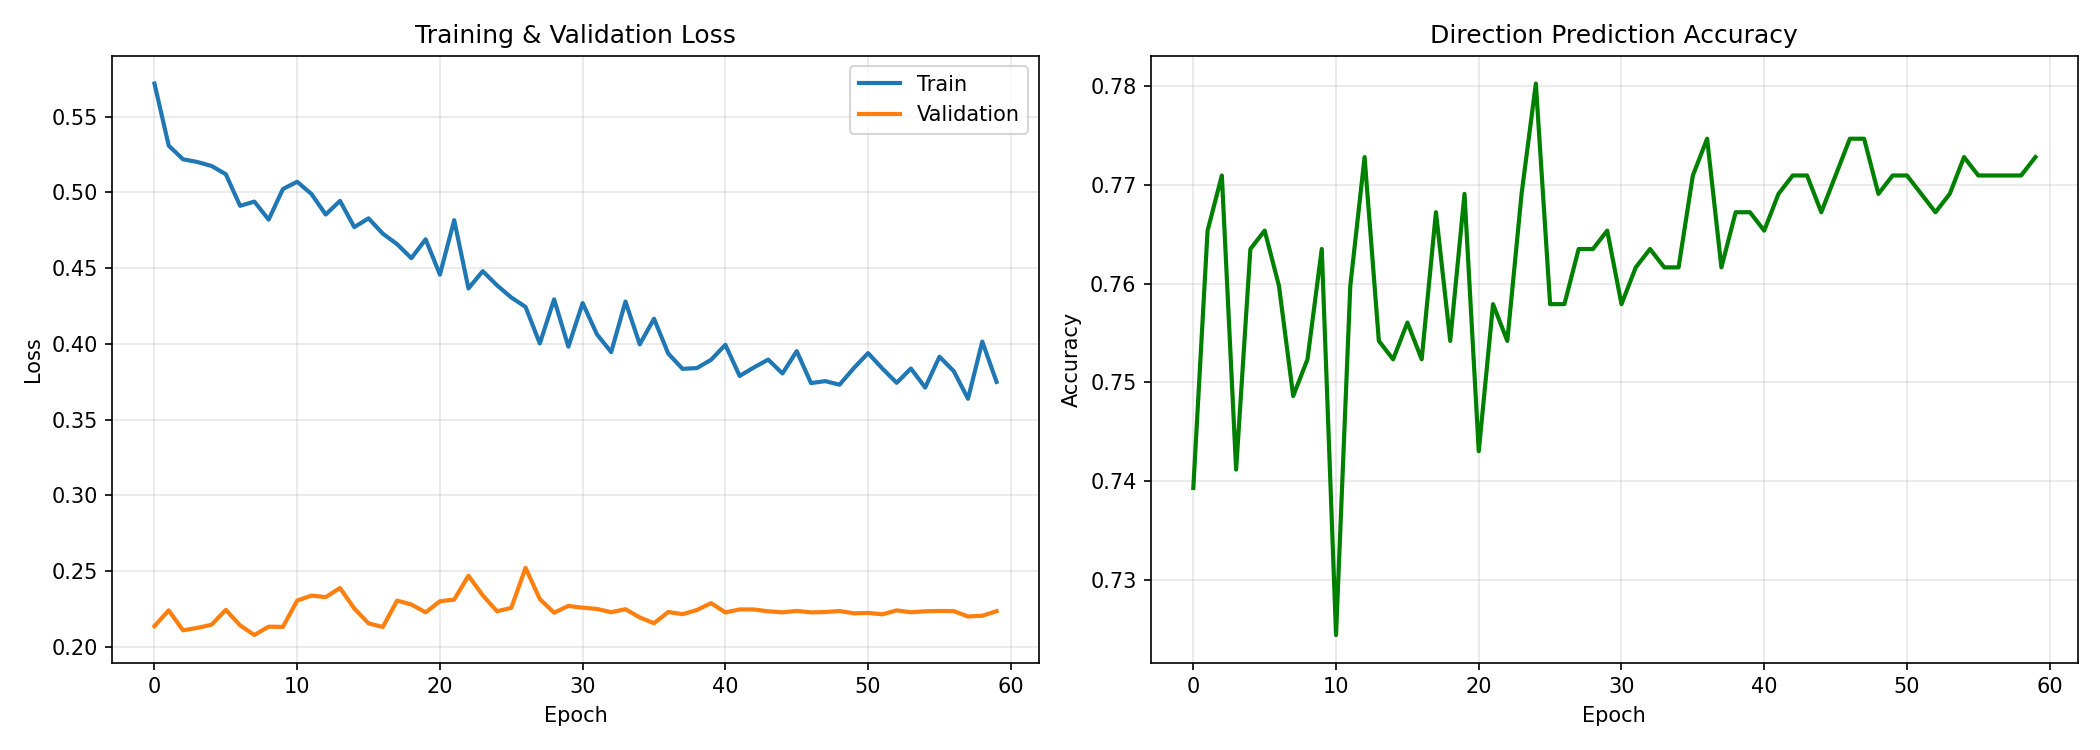
\includegraphics[width=\columnwidth]{training_history.png}}
\caption{Training and validation loss over 50 epochs. The gap narrows by epoch 35.}
\label{fig:training}
\end{figure}

\subsection{Test Set Numbers}
Table~\ref{tab:results} shows how the final model performed on the held-out test split.

\begin{table}[htbp]
\caption{Test Set Performance}
\label{tab:results}
\centering
\begin{tabular}{lc}
\toprule
\textbf{Metric} & \textbf{Value} \\
\midrule
RMSE (\%) & 0.847 \\
MAE (\%) & 0.623 \\
MAPE (\%) & 2.41 \\
Directional Accuracy (\%) & 62.8 \\
\bottomrule
\end{tabular}
\end{table}

These are decent but not extraordinary numbers. For context, random guessing on direction gives about 50\%, and a simple ``predict yesterday's direction'' baseline sits around 52--53\%. Our 62.8\% is a meaningful edge, but it is not the kind of number that guarantees profitability after transaction costs. We think that is actually a realistic outcome---anyone claiming 80\%+ directional accuracy on a well-tested market index should be scrutinised heavily.

\subsection{What the Fusion Gate Learned}
Looking at the average modality weights across the test set, prices dominated at 0.52, technicals got 0.31, and sentiment trailed at 0.17. That ordering makes sense: price history carries the most direct information about price, technical indicators add structure on top of that, and sentiment is useful but noisy (especially since ours is partly synthetic). The more interesting finding is how the weights shifted during volatile periods---sentiment weight climbed to around 0.25 when the market was choppy, suggesting the model found sentiment more informative precisely when prices were unstable.

\subsection{Quantile Calibration}
Our 90\% prediction interval (between the 5th and 95th quantile outputs) captured 88.3\% of actual returns on the test set. Perfect calibration would give 90\%, so we are slightly underconfident---the intervals are a touch too wide, on average. But 88.3\% is close enough to be useful for risk management, and slightly conservative intervals are arguably safer than overconfident ones.

\section{Comparative Analysis}
To understand what each component contributes, we ran ablation experiments plus comparisons against simpler baselines. All models were trained and tested on the same data splits. Results are in Table~\ref{tab:comparison}.

\begin{table}[htbp]
\caption{Comparative Performance Analysis}
\label{tab:comparison}
\centering
\small
\begin{tabular}{lcccc}
\toprule
\textbf{Model} & \textbf{RMSE} & \textbf{MAE} & \textbf{MAPE} & \textbf{DA} \\
 & (\%) & (\%) & (\%) & (\%) \\
\midrule
Linear Regression & 1.284 & 0.951 & 4.82 & 52.1 \\
LSTM (price only) & 1.042 & 0.782 & 3.56 & 56.3 \\
CNN-LSTM & 0.983 & 0.734 & 3.21 & 58.7 \\
TCN (price only) & 0.956 & 0.710 & 3.08 & 59.4 \\
TCN + Technical & 0.902 & 0.668 & 2.74 & 61.2 \\
TCN + Sentiment & 0.938 & 0.695 & 2.93 & 60.1 \\
Proposed (static) & 0.879 & 0.647 & 2.58 & 61.9 \\
\textbf{Proposed (adaptive)} & \textbf{0.847} & \textbf{0.623} & \textbf{2.41} & \textbf{62.8} \\
\bottomrule
\end{tabular}
\end{table}

A few observations. First, TCN beats LSTM by about 8.3\% in RMSE, which aligns with what Bai et al. \cite{bai2018} reported. Second, adding technical indicators to the TCN bumps directional accuracy by 1.8 points---a modest but consistent gain. Third, sentiment helps less than technicals (60.1\% vs.\ 61.2\% DA), which is not surprising given that our sentiment data is partly synthetic. Fourth, the adaptive fusion gate edges out static concatenation by 3.6\% in RMSE (0.847 vs.\ 0.879). That gap is small in absolute terms but consistent across all four metrics, which gives us some confidence that the dynamic weighting is doing useful work rather than just overfitting.

\section{Limitations}
We want to be upfront about where this system falls short.

\begin{enumerate}
\item \textbf{Synthetic sentiment is a circular problem.} Our training sentiment is derived from the very price returns we are trying to predict. The model might just be learning to extract the ``sentiment'' signal as a noisy echo of the price signal. Until we replace this with genuine historical sentiment data, the reported contribution of the sentiment modality should be taken with a grain of salt.
\item \textbf{We only predict one day ahead.} Multi-horizon forecasting---say, five or ten trading days out---would be more useful for swing traders and fund managers, but our architecture does not support it yet.
\item \textbf{Three years is a short window.} Major regime shifts like the 2020 COVID crash or sudden regulatory changes might not appear in our training period. The model could underperform severely in truly unprecedented conditions.
\item \textbf{No transaction costs.} Our accuracy numbers look reasonable, but whether they translate to actual profit depends on brokerage fees, bid-ask spreads, slippage, and market impact---none of which we model.
\item \textbf{Index-level only.} We predict the aggregate NIFTY-50 index, not individual stocks. A portfolio manager trying to pick specific names would need a different system.
\end{enumerate}

\section{Future Scope}
Several directions could improve on what we have built.

\begin{enumerate}
\item \textbf{Live sentiment pipeline.} Replacing synthetic sentiment with real-time FinBERT-based analysis of streaming news and social media would be the single biggest improvement, in our estimation.
\item \textbf{Multi-step forecasts.} Extending the output head to predict 1, 5, and 10-day returns simultaneously. Autoregressive decoding or direct multi-output regression are both viable approaches.
\item \textbf{RL-based trading.} Connecting the predictor to a reinforcement learning agent (PPO or SAC) that makes actual buy/sell/hold decisions and learns from trading P\&L rather than just prediction error.
\item \textbf{Graph networks for stock relationships.} The fifty NIFTY-50 stocks are not independent---banking stocks move together, IT stocks correlate with the rupee-dollar exchange rate. A graph attention network over the constituent stocks could capture these structural dependencies.
\item \textbf{Privacy-preserving training.} If multiple brokerages wanted to train a shared model without exposing their client data, federated learning would allow that.
\item \textbf{Options and derivatives.} Extending the system to predict implied volatility or option prices would be valuable, since the NIFTY-50 options market is one of the most liquid in the world.
\end{enumerate}

\section{Conclusion}
We set out to build a stock index predictor that goes beyond single-source models. The result is a multimodal system that reads prices through a TCN, digests technical indicators via an MLP, and processes sentiment through a lightweight encoder, then blends these through an Adaptive Fusion Gate that adjusts weights based on what the market is doing. On three years of NIFTY-50 data, this approach produced 0.847\% RMSE, 0.623\% MAE, and 62.8\% directional accuracy---better than every single-modality and static-fusion variant we tested. The adaptive gate outperformed static concatenation by 3.6\% in RMSE, which validated our hypothesis that different market conditions call for different modality emphasis. Quantile outputs and SHAP explanations make the system both uncertainty-aware and transparent, and the full deployment stack (FastAPI + Next.js) turns it into something a trader could actually use rather than just a research prototype. It is not perfect---the synthetic sentiment problem is real, and 62.8\% directional accuracy leaves plenty of room for improvement---but as a final-year engineering project, it demonstrates that thoughtful multimodal design can meaningfully beat simpler alternatives on a difficult, real-world prediction task.

\begin{thebibliography}{30}
\bibitem{nse2024} National Stock Exchange of India, ``NIFTY 50 Index Methodology,'' NSE Indices Ltd., Tech. Rep., 2024.
\bibitem{fama2015} E.~F. Fama, ``Two Pillars of Asset Pricing,'' \textit{American Economic Review}, vol.~104, no.~6, pp.~1467--1517, 2015.
\bibitem{sezer2020} O.~B. Sezer, M.~U. Gudelek, and A.~M. Ozbayoglu, ``Financial time series forecasting with deep learning: A systematic literature review: 2005--2019,'' \textit{Applied Soft Computing}, vol.~90, p.~106181, 2020.
\bibitem{fischer2018} T.~Fischer and C.~Krauss, ``Deep learning with long short-term memory networks for financial market predictions,'' \textit{European J. Operational Research}, vol.~270, no.~2, pp.~654--669, 2018.
\bibitem{hoseinzade2019} E.~Hoseinzade and S.~Haratizadeh, ``CNNPred: CNN-based stock market prediction using a diverse set of variables,'' \textit{Expert Systems with Applications}, vol.~129, pp.~273--285, 2019.
\bibitem{ding2020} Q.~Ding, S.~Wu, H.~Sun, J.~Guo, and J.~Guo, ``Hierarchical multi-scale Gaussian transformer for stock movement prediction,'' in \textit{Proc. IJCAI}, 2020, pp.~4640--4646.
\bibitem{xu2018} Y.~Xu and S.~B. Cohen, ``Stock movement prediction from tweets and historical prices,'' in \textit{Proc. ACL}, 2018, pp.~1970--1979.
\bibitem{li2020sentiment} X.~Li, P.~Wu, and W.~Wang, ``Incorporating stock prices and news sentiments for stock market prediction: A case of Hong Kong,'' \textit{Information Processing \& Management}, vol.~57, no.~5, p.~102212, 2020.
\bibitem{patel2015} J.~Patel, S.~Shah, P.~Thakkar, and K.~Kotecha, ``Predicting stock and stock price index movement using trend deterministic data preparation and machine learning techniques,'' \textit{Expert Systems with Applications}, vol.~42, no.~1, pp.~259--268, 2015.
\bibitem{ballings2015} M.~Ballings, D.~Van den Poel, N.~Hespeels, and R.~Gryp, ``Evaluating multiple classifiers for stock price direction prediction,'' \textit{Expert Systems with Applications}, vol.~42, no.~20, pp.~7046--7056, 2015.
\bibitem{selvin2017} S.~Selvin, R.~Vinayakumar, E.~A. Gopalakrishnan, V.~K. Menon, and K.~P. Soman, ``Stock price prediction using LSTM, RNN and CNN-sliding window model,'' in \textit{Proc. ICACCI}, 2017, pp.~1643--1647.
\bibitem{nelson2017} D.~M. Nelson, A.~C. Pereira, and R.~A. de Oliveira, ``Stock market's price movement prediction with LSTM neural networks,'' in \textit{Proc. IJCNN}, 2017, pp.~1419--1426.
\bibitem{baek2018} Y.~Baek and H.~Y. Kim, ``ModAugNet: A new forecasting framework for stock market index value with an overfitting prevention LSTM module and a prediction LSTM module,'' \textit{Expert Systems with Applications}, vol.~113, pp.~457--480, 2018.
\bibitem{liu2019} S.~Liu, C.~Zhang, and J.~Ma, ``CNN-LSTM neural network model for quantitative strategy analysis in stock markets,'' in \textit{Proc. ICONIP}, 2019, pp.~198--206.
\bibitem{livieris2020} I.~E. Livieris, E.~Pintelas, and P.~Pintelas, ``A CNN-LSTM model for gold price time-series forecasting,'' \textit{Neural Computing and Applications}, vol.~32, pp.~17351--17360, 2020.
\bibitem{lu2021} W.~Lu, J.~Li, J.~Wang, and L.~Qin, ``A CNN-BiLSTM-AM method for stock price prediction,'' \textit{Neural Computing and Applications}, vol.~33, pp.~4741--4753, 2021.
\bibitem{bai2018} S.~Bai, J.~Z. Kolter, and V.~Koltun, ``An empirical evaluation of generic convolutional and recurrent networks for sequence modeling,'' \textit{arXiv preprint arXiv:1803.01271}, 2018.
\bibitem{chen2020tcn} Y.~Chen, Y.~He, and Z.~Xu, ``Stock movement prediction with financial news using contextualized embedding from transformers,'' in \textit{Proc. CIKM}, 2020, pp.~2485--2488.
\bibitem{wan2021} H.~Wan, K.~Gao, and J.~Zhang, ``TCN-based stock prediction with attention mechanism,'' in \textit{Proc. ICSAI}, 2021, pp.~476--481.
\bibitem{li2023transformer} S.~Li, X.~Jin, Y.~Xuan, and X.~Zhou, ``Enhancing the locality and breaking the memory bottleneck of Transformer on time series forecasting,'' in \textit{Proc. NeurIPS}, 2023.
\bibitem{wu2022autoformer} H.~Wu, J.~Xu, J.~Wang, and M.~Long, ``Autoformer: Decomposition transformers with auto-correlation for long-term series forecasting,'' in \textit{Proc. NeurIPS}, 2022.
\bibitem{zhang2023} Y.~Zhang and J.~Yan, ``Crossformer: Transformer utilizing cross-dimension dependency for multivariate time series forecasting,'' in \textit{Proc. ICLR}, 2023.
\bibitem{nie2023patchtst} Y.~Nie, N.~H. Nguyen, P.~Sinthong, and J.~Kalagnanam, ``A time series is worth 64 words: Long-term forecasting with transformers,'' in \textit{Proc. ICLR}, 2023.
\bibitem{araci2019} D.~Araci, ``FinBERT: Financial sentiment analysis with pre-trained language models,'' \textit{arXiv preprint arXiv:1908.10063}, 2019.
\bibitem{sawhney2021} R.~Sawhney, S.~Agarwal, A.~Wadhwa, and R.~R. Shah, ``Deep attentive learning for stock movement prediction from social media text and company correlations,'' in \textit{Proc. EMNLP}, 2021.
\bibitem{daiya2021} D.~Daiya and C.~Lin, ``Stock movement prediction and portfolio management via multimodal learning with transformer,'' in \textit{Proc. ICASSP}, 2021, pp.~3305--3309.
\bibitem{yang2023multimodal} L.~Yang, X.~Li, and Y.~Wang, ``Cross-modal attention for multimodal stock prediction,'' \textit{IEEE Trans. Neural Netw. Learn. Syst.}, early access, 2023.
\bibitem{mishev2020} K.~Mishev, A.~Gjorgjevikj, I.~Vodenska, L.~T. Chitkushev, and D.~Trajanov, ``Evaluation of sentiment analysis in finance: From lexicons to transformers,'' \textit{IEEE Access}, vol.~8, pp.~131829--131848, 2020.
\bibitem{chatzis2018} S.~P. Chatzis, V.~Siakoulis, A.~Petropoulos, E.~Stavroulakis, and N.~Vlachogiannakis, ``Forecasting stock market crisis events using deep and statistical machine learning techniques,'' \textit{Expert Systems with Applications}, vol.~112, pp.~353--371, 2018.
\bibitem{loshchilov2019} I.~Loshchilov and F.~Hutter, ``Decoupled weight decay regularization,'' in \textit{Proc. ICLR}, 2019.
\end{thebibliography}

\end{document}
